\section{Methodology}
\subsection{Data description and expected outputs}

\begin{figure}[h!]
    \centering
    % First image
    \begin{subfigure}[b]{0.3\textwidth} % Adjust width as needed for spacing
        \centering
        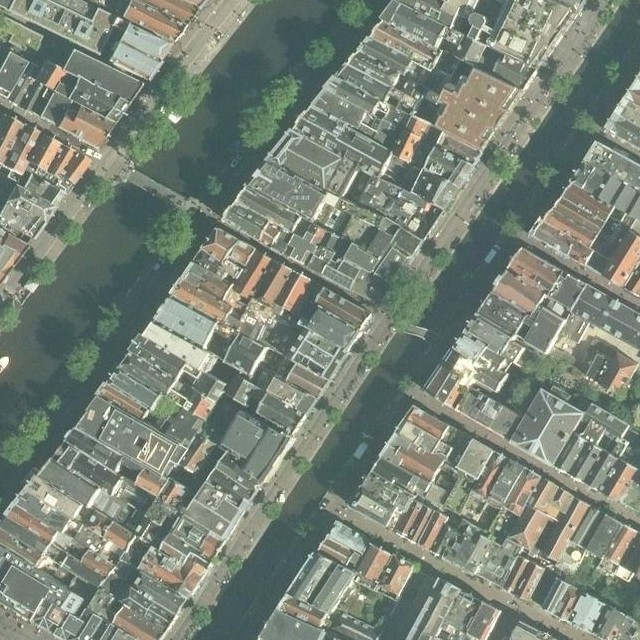
\includegraphics[width=\linewidth, height=\linewidth, keepaspectratio]{figures/methods/RGB_zone0.jpeg}
        \caption{Aerial RGB}
        \label{fig:methods_rgb}
    \end{subfigure}
    \hfill % Adds horizontal space between subfigures
    % Second image
    \begin{subfigure}[b]{0.3\textwidth}
        \centering
        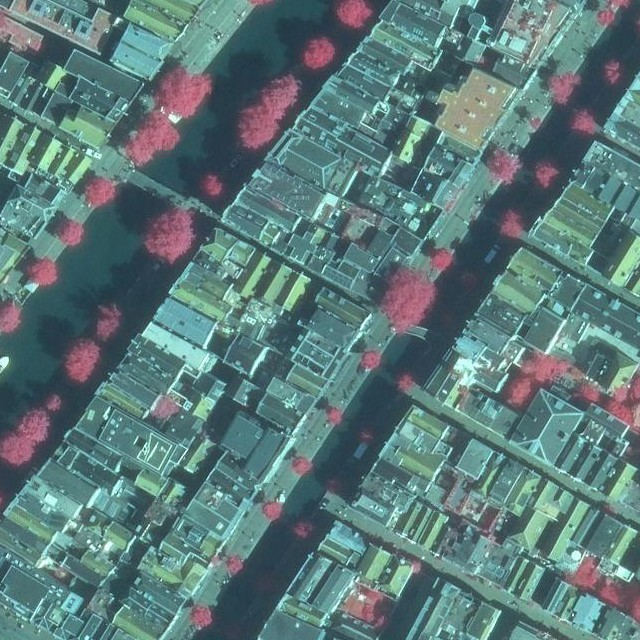
\includegraphics[width=\linewidth, height=\linewidth, keepaspectratio]{figures/methods/CIR_zone0.jpeg}
        \caption{Aerial CIR (Infrared)}
        \label{fig:methods_cir}
    \end{subfigure}
    \hfill % Adds horizontal space between subfigures
    % Third image
    \begin{subfigure}[b]{0.3\textwidth}
        \centering
        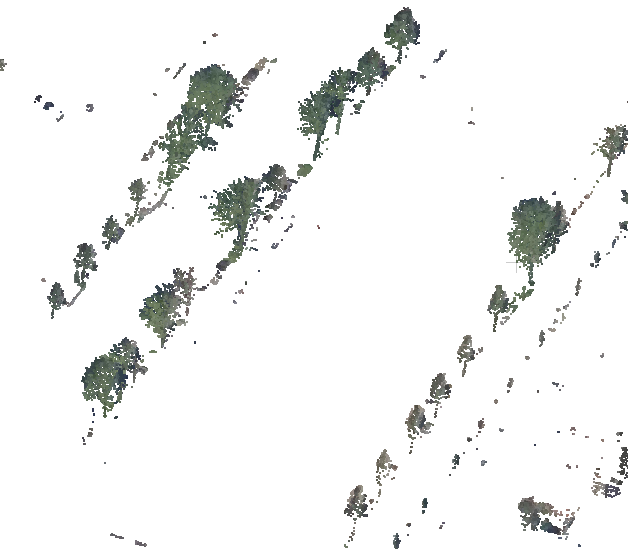
\includegraphics[width=\linewidth, height=\linewidth, keepaspectratio]{figures/methods/tree_viz.png}
        \caption{Vegetation Point Cloud}
        \label{fig:image3}
    \end{subfigure}
    \caption{Comparision of input data sources}
    \label{fig:three_images}
\end{figure}

This study uses complementary remote sensing data covering Amsterdam's urban area. High-resolution aerial imagery (0.25m) incorporating Near-Infrared (NIR) bands was acquired during the summer growing season (July 2023) to capture vegetation at peak foliage. LiDAR point cloud data with a density of 25 points/m² provides three-dimensional structural information, collected during the same temporal window to ensure correspondence with the aerial imagery. These datasets were supplemented with municipal tree inventory records containing genus information for 267,974 trees across diverse urban contexts.

% Global Availability
%%Add more here
While high-resolution aerial imagery is increasingly available through municipal open data portals, LiDAR coverage varies substantially. Our framework accommodates variable point densities (5-20 points/m²) through adaptive voxel sizing, enabling application in regions with less dense LiDAR coverage.

%% CHM and NDVI Rasters !!
% \begin{figure}[h!]
%     \centering
%     % First image
%     \begin{subfigure}[b]{0.48\textwidth} % Adjust width as needed for spacing
%         \centering
%         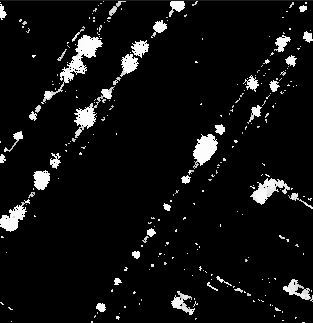
\includegraphics[width=\linewidth, height=\linewidth, keepaspectratio]{figures/methods/chm.png}
%         \caption{Visualization of Canopy Height Model (CHM)}
%         \label{fig:chm}
%     \end{subfigure}
%     \hfill % Adds horizontal space between subfigures
%     % Second image
%     \begin{subfigure}[b]{0.48\textwidth}
%         \centering
%         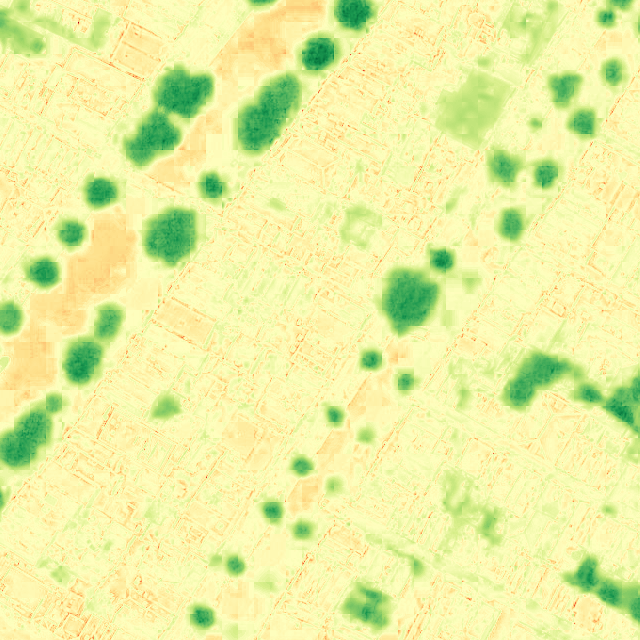
\includegraphics[width=\linewidth, height=\linewidth, keepaspectratio]{figures/methods/02_ndvi_data.png}
%         \caption{Visualization of Normalized Difference Vegetation Index (NDVI)}
%         \label{fig:ndvi}
%     \end{subfigure}
%     \caption{Preprocessed rasters for vegetation detection}
%     \label{fig:preproc_rasters}
% \end{figure}

% Data PreProcessing Pipeline
The data preprocessing pipeline involved three key steps: vegetation classification, Canopy Height Model (CHM) generation, and Normalized Difference Vegetation Index (NDVI) calculation. Raw LiDAR point clouds were manually classified based on HSV (Hue, Saturation, Value) color values to isolate vegetation from the colored point cloud, leveraging distinct color characteristics in the HSV color space for accurate separation. A 0.5m-resolution CHM was then generated by subtracting a Digital Terrain Model (DTM) from a Digital Surface Model (DSM), with noise filtering applied to ensure vertical accuracy. NDVI was calculated from aerial imagery at 0.25m resolution using the formula (NIR - Red)/(NIR + Red).

To improve the robustness of our tree segmentation model and reduce false positives in non-vegetated areas, we applied a NDVI-based contrast enhancing pipeline on aerial images (Supplementary Figure 1). Specifically, pixels with NDVI values below 0.0 were progressively darkened using a linear attenuation function with a minimum brightness factor of 0.4. This was followed by partial desaturation of the same regions, blending 50\% toward grayscale to suppress color cues in non-vegetated zones. Finally, a Gaussian blur was applied to low-NDVI areas to reduce distracting texture and emphasize vegetated regions. This approach preserves the overall image structure while subtly guiding the model's attention toward vegetated areas without introducing unnatural masking artifacts.


% Output
Our methodology produces four primary data products: (1) individual tree crown polygons matched with genus attribution from municipality database when available, (2) tree morphological parameters (height and crown diameter), (3) high-resolution LAI maps at 0.5m² resolution, and (4) a predictive model for estimating LAI from tree morphology and genus. These outputs are delivered in standard GIS formats (GeoJSON, GeoTIFF) to maximize interoperability with existing urban planning tools.

\subsection{Tree Crown Segmentation}
% Segmentation and Overlay
% Insert Detection Bounding Box Figure
To detect individual trees from high-resolution aerial imagery, we employed the DeepForest model % TODO: Add DeepForest citation to references.bib
, a deep learning-based object detection framework specifically designed for tree crown delineation. DeepForest utilizes a RetinaNet architecture % TODO: Add RetinaNet citation to references.bib
 with a ResNet-50 backbone and is trained on a diverse set of forest types using RGB imagery. In our workflow, we leveraged the pre-trained model provided by DeepForest, which identifies individual tree crowns by predicting bounding boxes directly from RGB image tiles. This approach allows for accurate tree detection without the need for multispectral or LiDAR data, making it suitable for generalization in context where Aerial Lidar Scan data might not be available. The model outputs were further refined through confidence thresholding and non-maximum suppression to eliminate duplicate detections.


\subsection{Voxel-based Leaf Area Index Estimation}\label{LAI}
% Leaf Area Index Estimation
Our LAI calculation leverages a voxelization technique implemented through the LeafR package % TODO: Add Almeida et al. (2019) LeafR package citation to references.bib
, which processes LiDAR point cloud data by transforming it into a voxel-based representation of the canopy structure. The space containing each tree crown is divided into cubic voxels, with the ratio of vegetation points to total points within each voxel calculated and calibrated against Beer-Lambert light extinction principles to estimate Leaf Area Density (LAD). LAD profiles are generated using the MacArthur-Horn method % TODO: Add MacArthur-Horn method citation to references.bib
, which analyzes the probability of LiDAR pulses penetrating the canopy and calculates the return ratio from each vertical layer, providing a systematic understanding of leaf distribution. The LAI is derived by vertically integrating the LAD profile, summing leaf area density values across the canopy height to provide a comprehensive measure of the total one-sided leaf area per unit ground surface area. The selected 0.5m³ resolution balances computational efficiency with accuracy, enabling non-destructive, scalable LAI estimation for individual trees or entire urban forests. This method could also support temporal analysis through repeated LiDAR scans, facilitating the tracking of LAI changes over time, seasons, or in response to environmental factors.

\subsection{Machine Learning Pipeline for LAI Prediction}

% \subsubsection{Feature Engineering}

We constructed a comprehensive feature set encompassing 58 variables across six categories to capture morphological, spectral, and contextual information relevant to LAI prediction.

\textbf{Base morphological features} (13 features) included tree height statistics (mean, minimum, maximum, standard deviation, median), crown dimensions (diameter, area, perimeter), structural ratios (height-to-crown ratio), and detection confidence scores from the segmentation algorithm.

\textbf{Spectral features} (6 features) comprised NDVI statistics within individual tree crowns (mean, minimum, maximum, standard deviation), neighborhood spectral context (average NDVI within 20m radius), and spatial NDVI variability.

\textbf{Allometric features} (8 features) applied power law and logarithmic transformations following biological scaling theory: height$^2$, crown\_diameter$^2$, log(height), log(crown\_area), and the height-diameter power term $(height/diameter)^{1.5}$.

\textbf{NDVI interaction terms} (7 features) captured spectral-structural relationships through multiplicative interactions (NDVI $\times$ height, NDVI $\times$ crown\_diameter) and derived indices (canopy vigor per unit height: NDVI/height).

\textbf{Categorical features} (6 features) encoded height classes as binary indicators ($<$5m, 5--10m, 10--15m, 15--20m, 20--25m, $>$25m) to capture potential threshold effects in height-LAI relationships.

\textbf{Species and geospatial features} (10 features) included leaf habit (deciduous/coniferous), species groupings (major genera vs. ``unknown''), nearest neighbor distance, local tree density (counts within 15m, 30m, 50m radii), and edge proximity indicators.

\textbf{Feature preprocessing:} Continuous features were standardized using z-score normalization ($\mu=0$, $\sigma=1$) fitted on the training set and applied identically to validation and test sets to prevent data leakage. Categorical variables were one-hot encoded for linear models and handled natively by tree-based algorithms. Missing values in species features were assigned to an ``unknown'' category; missing morphological features (0.3\% of observations) were median-imputed using training set statistics.

% \subsubsection{Data Partitioning}

The dataset (N=7,085) was partitioned into training (70\%, N=4,959), validation (15\%, N=1,063), and test (15\%, N=1,063) sets using stratified random sampling. Stratification was performed on LAI quintiles to maintain representative target distributions across splits, with secondary stratification on height tertiles within each LAI stratum. A fixed random seed (seed=42) ensured reproducibility.

% \subsubsection{Model Selection and Architecture}

We evaluated eight predictive models representing diverse algorithmic approaches:

\textbf{(1) Linear Regression:} Ordinary least squares baseline to assess linear relationships without regularization (scikit-learn \texttt{LinearRegression}).

\textbf{(2) Ridge Regression:} L2-regularized linear model with penalty $\alpha\|\mathbf{w}\|_2^2$. Hyperparameter $\alpha$ was tuned via 5-fold cross-validation over $\{0.01, 0.1, 1, 10, 100\}$.

\textbf{(3) Lasso Regression:} L1-regularized linear model with penalty $\alpha\|\mathbf{w}\|_1$ for implicit feature selection. Hyperparameter $\alpha$ was tuned over $\{0.001, 0.01, 0.1, 1, 10\}$.

\textbf{(4) Random Forest:} Bagging ensemble of 500 decision trees with randomized feature subsets. Hyperparameters were tuned via grid search: \texttt{max\_depth} $\in \{10, 20, 30, \text{None}\}$, \texttt{min\_samples\_leaf} $\in \{1, 2, 4\}$, \texttt{max\_features} $\in \{\text{sqrt}, \text{log2}, 0.3\}$. Final configuration: \texttt{max\_depth}=20, \texttt{min\_samples\_leaf}=2, \texttt{max\_features}=sqrt.

\textbf{(5) XGBoost:} Gradient boosted decision trees with L1/L2 regularization. Hyperparameters were optimized via Bayesian optimization (Optuna, 100 trials) with objective function minimizing validation RMSE. Search ranges: \texttt{learning\_rate} [0.01, 0.3], \texttt{max\_depth} [3, 10], \texttt{n\_estimators} [100, 1000], \texttt{subsample} [0.6, 1.0], \texttt{colsample\_bytree} [0.6, 1.0], \texttt{reg\_alpha} [0, 1], \texttt{reg\_lambda} [0, 10]. Early stopping with patience=50 rounds prevented overfitting. Final configuration: \texttt{learning\_rate}=0.08, \texttt{max\_depth}=6, \texttt{n\_estimators}=450, \texttt{subsample}=0.85.

\textbf{(6) Support Vector Regression (SVR):} Radial basis function kernel with hyperparameters $C$ (regularization) $\in \{0.1, 1, 10, 100\}$, $\epsilon$ (tube width) $\in \{0.01, 0.1, 0.5\}$, and $\gamma$ (kernel coefficient) $\in \{\text{scale}, \text{auto}, 0.001, 0.01\}$ tuned via grid search.

\textbf{(7) Neural Network:} Multi-layer perceptron with architecture [100, 50] (two hidden layers, ReLU activation), dropout rate 0.2, Adam optimizer (learning rate=0.001). Training used batch size 32, maximum 500 epochs with early stopping (patience=20 on validation loss).

\textbf{(8) Allometric Baseline:} Traditional forestry model: $\text{LAI} = \alpha \times H^\beta \times \text{CD}^\gamma$, where $H$ is height and CD is crown diameter. Parameters $(\alpha, \beta, \gamma)$ were estimated via non-linear least squares on training data, providing an ecological benchmark.

% \subsubsection{Model Training and Evaluation}

Models were trained exclusively on the training set, with hyperparameter tuning guided by validation set performance. The test set remained completely held out until final evaluation to provide unbiased performance estimates.

\textbf{Performance metrics:} We evaluated models using three complementary metrics: (1) coefficient of determination ($R^2 = 1 - \text{SS}_{\text{res}}/\text{SS}_{\text{tot}}$) measuring explained variance, (2) root mean squared error (RMSE = $\sqrt{\sum(y_{\text{pred}} - y_{\text{true}})^2 / n}$) in LAI units, and (3) mean absolute error (MAE = $\sum|y_{\text{pred}} - y_{\text{true}}| / n$) providing robust, interpretable prediction error.

% \textbf{Statistical significance testing:} Pairwise model comparisons employed paired t-tests on performance estimates from 5-fold stratified cross-validation repeated 10 times (50 samples per model). Stratification maintained LAI quintile distributions within folds. Bonferroni correction adjusted significance threshold to $\alpha = 0.05/28 = 0.0018$ for multiple comparisons across 8 models.

% \textbf{Residual analysis:} We examined residual patterns via predicted-vs-actual scatter plots, residual-vs-predicted plots, and Q-Q plots to assess normality. Heteroscedasticity was tested using the Breusch-Pagan test. Spatial autocorrelation in residuals was quantified via Moran's $I$ statistic with a 10km distance band to detect systematic spatial prediction biases.

% \subsubsection{Feature Importance Analysis}

\textbf{XGBoost gain-based importance:} Feature importance was computed as the average information gain across all tree splits utilizing each feature, normalized to sum to 1.0. This quantifies each feature's contribution to reducing prediction error.

\textbf{Random Forest importance:} Mean decrease in Gini impurity provided an independent importance ranking. Spearman rank correlation between XGBoost and Random Forest rankings assessed consistency across algorithms.

% \textbf{SHAP values:} We applied SHapley Additive exPlanations % TODO: Add lundberg2017unified citation to references.bib (SHAP: Lundberg & Lee, 2017)
 to the XGBoost model for model-agnostic feature importance. Global importance was measured as mean absolute SHAP value per feature. SHAP dependence plots revealed interaction effects (e.g., NDVI $\times$ height) and non-linear relationships.

% \subsubsection{Feature Ablation Study}

To quantify the marginal contribution of engineered feature categories, we conducted a systematic ablation study. Eight feature configurations were evaluated: (1) \textit{All Features} (N=42, baseline), (2) \textit{Base Only} (N=13: height, crown, NDVI only), (3) \textit{Base + NDVI interactions} (N=19), (4) \textit{Base + Allometric} (N=23), (5) \textit{No Species} (N=39), (6) \textit{No Allometric} (N=34), (7) \textit{No NDVI Interactions} (N=38), (8) \textit{No Geospatial} (N=38). For each configuration, an XGBoost model was trained using identical hyperparameters, and performance was evaluated on the validation set. Performance degradation ($\Delta R^2$) relative to the full feature set quantified each category's importance.

% \subsubsection{Species-Specific Performance}

We analyzed model performance stratified by species to identify taxa-specific prediction patterns. Only species with $N \geq 20$ test samples were included to ensure statistical reliability. Performance metrics ($R^2$, RMSE, MAE) were calculated separately for each species group. 
% One-way ANOVA tested whether performance varied significantly across species ($\alpha=0.05$), with Tukey HSD post-hoc tests for pairwise comparisons if significant.

% \subsubsection{Software and Reproducibility}

All analyses were performed in Python 3.9.7 using scikit-learn 1.0.2 (linear models, Random Forest, SVR, Neural Network), XGBoost 1.5.0, SHAP 0.40.0, and Optuna 2.10.0 for hyperparameter optimization. Random seeds were fixed (seed=42) across all stochastic processes (data splitting, model initialization, cross-validation) to ensure reproducibility. Computations were performed on an Intel Core i7, Nvidia GeForce RTX 3090 (32GB RAM). Code and trained models will be made publicly available upon publication at [repository URL].
% \subsubsection{Model Selection and Architecture}
% % Model Selection and Architecture
% To enable LAI prediction in areas with limited LiDAR coverage, we developed a machine learning model to estimate LAI from tree morphological parameters and genus information. After evaluating multiple algorithms (Linear Regression, Support Vector Regression, Gradient Boosting), Random Forest Regression demonstrated superior performance (lowest RMSE and highest R²) and was selected as the final model. The model architecture included ?? decision trees with a maximum depth of ?? to balance model complexity with generalization capability. Five-fold cross-validation was implemented to ensure robustness and assess model stability.

% \subsubsection{Feature Engineering}
% % Training Parameters and Feature Engineering
% The model was trained on data from ?? trees spanning ?? genera common in urban environments. Input features included morphological parameters and genus encoded as categorical variables using one-hot encoding. Feature importance analysis revealed that tree height (??), crown volume (??), and genus (??) were the strongest predictors of LAI. Model hyperparameters were optimized using a grid search with cross-validation, resulting in a minimum samples split of ? and a minimum samples leaf of ?. The final model achieved an R² of ? and RMSE of ? m²/m² on the test set (? of data held out from training).

% \subsubsection{Evaluation Metrics}

% We employed LiDAR-based LAI estimates as training targets from \ref{LAI} for our machine learning regression model. The voxelization-derived LAI values were paired with corresponding morphological features tree height, crown diameter, and height to crown diameter ratios) extracted from the aerial imagery and CHM, as well as NDVI computed from the NIR band. This approach leverages the physically-grounded LAI estimates from the MacArthur-Horn method as ground truth, circumventing the need for time-consuming field validation while simultaneously generating training data across the entire detected tree population. Model performance was assessed using five-fold cross-validation to guard against overfitting and provide robust estimates of generalization capability. To further validate model predictions beyond the training set, we separately retained $?\%$ of trees as a held-out test set, which was evaluated using the evaluation metrics described in section 2.2.3 (RMSE and R²). This multi-layered validation approach ensures that the resulting model captures the morphology-LAI relationships inherent in the LiDAR-derived estimates while maintaining sufficient independence to assess predictive reliability when applied to new tree crowns detected in regions where LiDAR coverage may be limited or unavailable.

